\section{Experiment}
In order to prove the effectiveness of spatial features, we test the features on NAME, NAME+BASE, NAME+BASE+BEST. We use LIBLINEAR, one of the most popular classification toolkits, to build a binary classifier for each category, and then combine the result of the classifiers to produce the final classification result.

In the following, we introduce our data set first, and start by testing features individually on different categories to show different strength of features on different categories, then we show the result after choosing the best combination of features for each category. In the last two parts, we combine the results of categories' binary classifiers to produce multi-label result for Level 1 category and Level 2 categories.

\subsection{Data set description}
In order to test spatial features, we select check-ins from Foursquare in cities of two different size: NewYork(7817 POIs, 20885 check-ins), Singapore(38394 POIs,367570 check-ins). We use category hierarchy from Foursquare, too, we show the first level categories and their percentage in the two data set in Table \ref{tab:CategoryInfo}, and later we also do experiments on second level category, which is more specified including 278 categories. Among the POIs, there are 15.9\% of NewYork and 11.5\% of Singapore that are with multiple labels. We show that spatial features influenced less by user check-ins and consistently show improvements over BASE features.

\begin{table}
% Table generated by Excel2LaTeX from sheet 'Sheet1'
\caption{Please write your table caption here}
\label{tab:CategoryInfo}
\begin{tabular}{|c|r|r|}
\hline
 & NewYork(7817) & Singapore(38394) \\
\hline
Arts \& Entertainment &       10\% &        5\% \\
\hline
College \& University &        3\% &        8\% \\
\hline
      Food &       40\% &       28\% \\
\hline
Nightlife Spot &       19\% &        4\% \\
\hline
Outdoors \& Recreation &        4\% &        6\% \\
\hline
Professional \& Other Places &       16\% &       18\% \\
\hline
 Residence &        4\% &       16\% \\
\hline
Shop \& Service &       18\% &       19\% \\
\hline
Travel \& Transport &        5\% &        9\% \\
\hline
\end{tabular}


\end{table}

\subsection{Features on different Categories}
We show different features' strength on different categories in Fig. \ref{fig:F1FeatureCate}. One thing to be noted here is that even some features do not work well on their own, they show some different aspects of the POI, thus still can improve result.

We start by seeing BASE feature's performance over others in different categories. BASE feature consists of user behavior analysis, it works very well on Nightlife Spot and Professional \& Other Places, which has typical time characteristic, at night and on weekday individually. However, it works not so well on places with less characteristic on time specifically, for example Arts \& Entertainment, Shop \& Service.

NB\_m feature showed relatively good result among all the categories, showing that most of the POIs appear at appropriate and typical neighborhood for them. Interesting fact about N\_k feature is that it will get significant better result than NB\_m when POIs of same category gathering ''purely"" together, such as College \& University and Residence, however not so good result when the category normally mixed with other categories, such as Nightlife Spot. When using N\_K feature alone, the performance rely largely on whether the POIs near are within the same category. LCD feature, which measures distance to different categories, on its own is a very weak feature. When using it alone, it will show accordance with N\_k feature. The reason is that LCD get small distance to the POIs with same category, thus has similar effect as N\_K feature. Region compare on total check-in and unique user have similar effect.


\begin{figure}[h]
\centering
\subfigure[Arts \& Entertainment]{
\label{fig:F1FeatureArt}
\epsfig{file=plot/Graph_Youer/FeatureF1ForCate_data/Arts_&_Entertainment_data.eps,width=0.3\columnwidth}
}
\subfigure[Shop \& Service]{
\epsfig{file=plot/Graph_Youer/FeatureF1ForCate_data/Shop_&_Service_data.eps,width=0.3\columnwidth}
}
\subfigure[Food]{
\epsfig{file=plot/Graph_Youer/FeatureF1ForCate_data/Food_data.eps,width=0.3\columnwidth}
}
\subfigure[Nightlife Spot]{
\epsfig{file=plot/Graph_Youer/FeatureF1ForCate_data/Nightlife_Spot_data.eps,width=0.3\columnwidth}
}
\subfigure[Outdoors \& Recreation]{
\epsfig{file=plot/Graph_Youer/FeatureF1ForCate_data/Outdoors_&_Recreation_data.eps,width=0.3\columnwidth}
}
\subfigure[Professional \& Other Places]{
\epsfig{file=plot/Graph_Youer/FeatureF1ForCate_data/Professional_&_Other_Places_data.eps,width=0.3\columnwidth}
}
\subfigure[College \& University]{
\epsfig{file=plot/Graph_Youer/FeatureF1ForCate_data/College_&_University_data.eps,width=0.3\columnwidth}
}
\subfigure[Residence]{
\epsfig{file=plot/Graph_Youer/FeatureF1ForCate_data/Residence_data.eps,width=0.3\columnwidth}
}
\subfigure[Travel \& Transport]{
\epsfig{file=plot/Graph_Youer/FeatureF1ForCate_data/Travel_&_Transport_data.eps,width=0.3\columnwidth}
}
\caption{F1 score for individual features on categories}
\label{fig:F1FeatureCate}
\end{figure}







\subsection{Choosing feature parameter and combination}
As mentioned above, different parameter would have different effect on classification of different categories.Moreover, different combinations of parameters will also result in different accuracy. Thus, we tried all possible combinations for different categories and choose the best one based on tune set, and get the experiment result on the test set.

In the experiment on NewYork's data, every category gets better result over NAME+BASE except Art \& Entertainment, which results from the imbalance from test set and tune set, the best combination we choose for Art for NewYork works very well on tune set while not so well on test set.

In the experiment on Singapore's data, all the categories get better result over NAME+BASE, which benefit from the abundant train data.

Concluding from the two results on each category, we find that adding up spatial features will help in identifying a POI's category, but which features to add depend on the characteristic of the particular category.

%\begin{figure}[h]
%\centering
%\subfigure[NewYork]{
%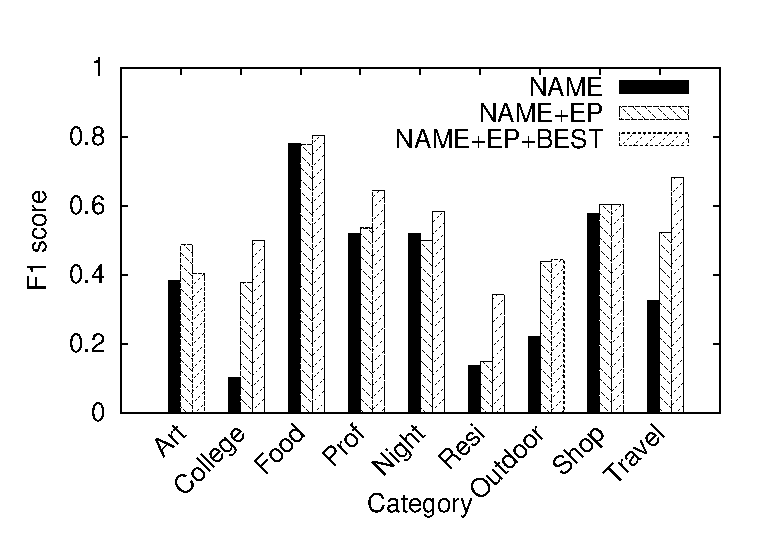
\epsfig{file=plot/Graph_Youer/NewYorkF1.eps,width=0.47\columnwidth}
%}
%\subfigure[Singapore]{
%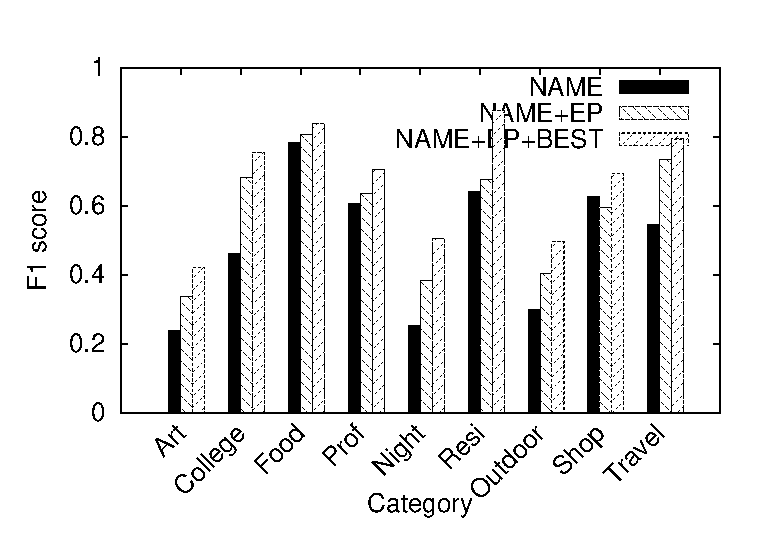
\epsfig{file=plot/Graph_Youer/SingaporeF1.eps,width=0.47\columnwidth}
%}
%\end{figure}

\begin{figure}[h]
\centering
% Use the relevant command to insert your figure file.
% For example, with the graphicx package use
  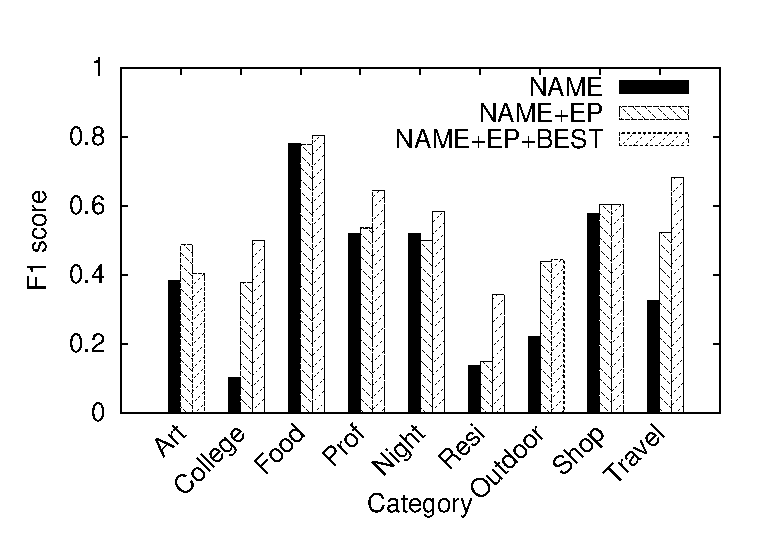
\epsfig{file=plot/Graph_Youer/NewYorkF1.eps,width=0.7\columnwidth}
% figure caption is below the figure
\caption{F1 score of different categories(NewYork)}
\label{fig:NewYorkF1}       % Give a unique label
\end{figure}
\begin{figure}[h]
\centering
% Use the relevant command to insert your figure file.
% For example, with the graphicx package use
  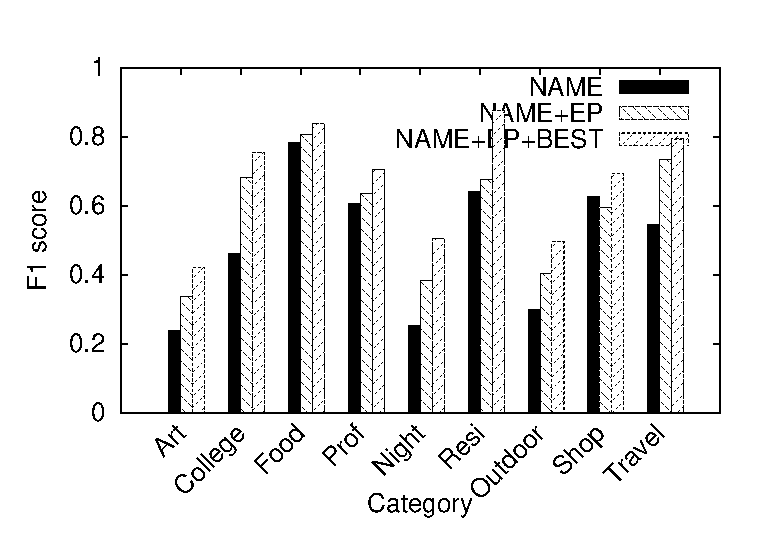
\epsfig{file=plot/Graph_Youer/SingaporeF1.eps,width=0.7\columnwidth}
% figure caption is below the figure
\caption{F1 score of different categories(Singapore)}
\label{fig:SingaporeF1}       % Give a unique label
\end{figure}

\subsection{Multi-label Classification Result}
We will get a prediction,indicating a 0-1 label for given category, and the probability output, indicating the probability of belonging to given category, from each category's classifier. We evaluate the prediction result by performing strict accuracy, precision and recall measure on multi-label classification. And we also produce a ranking list of the category label by probability output for each POI, we show ground-truth labels are ranked high in the ranking list to illustrate the reliability of candidate category labels we provide. We apply One-error, Coverage and average precision to measure the ranking list.
\subsubsection{Multi-label Performance Metrics}
\paragraph{Strict prediction measure} We define POI test set $T$ as a set of $|T|$ POI multi-label instances $(t_i, L_i)$, where $t_i$ is a POI, and $L_i$ is the ground-truth label set for $t_i$. The label(category) space $C$ consist of $|C|$ categories, for each category we have a binary classifier $BC_c, c \in C$. Each classifier have a 0-1 label for each instance $BC_j(t_i) = x, x \in {0,1}$, the final category prediction for $t_i$ is $P_i = \bigcup_{BC_c(t_i)=1} c \in C $,  Thus, we measure accuracy, precision and recall as follows.
\begin{description}
\centering
\item $Accuracy(T)=\frac{1}{|T|} \sum^{|T|}_{i=1} \frac{|L_i \cap P_i|}{|L_i \cup P_i|}$

\item $Precision(T)=\frac{1}{|T|} \sum^{|T|}_{i=1} \frac{|L_i \cap P_i|}{|P_i|}$

\item $Recall(T)=\frac{1}{|T|} \sum^{|T|}_{i=1} \frac{|L_i \cap P_i|}{|L_i|}$
\end{description}
\paragraph{Ranking list measure}
We further define probability of $t_i$ given category $c$ as $Pr_i(c)$. We have a permutation of C's items descending ordered by $Pr_i(c)$.
\begin{description}

\item[One-error:] Evaluation of whether ranked top category belongs to the ground-truth category set. $OneError = \frac{1}{|T|} \sum^{|T|}_{i=1}f([\arg\max_{c \in C} Pr_i(c)] \notin L_i$, for and predicate $\pi$, $f(\pi)$ equals 1 if $\pi$ holds and 0 otherwise.

\item[Coverage:] Evaluation of how many items should be seen on the list in order to cover all the ground-truth categories. We define $R_i(c)$ as the category c's rank in category ranking list of $t_i$. Thus  $Coverage = \frac{1}{|T|} \sum^{|T|}_{i=1} \max_{l \in L_i} R_i(l) -1$.

\item[Average Precision:] Evaluation of the ranking list considering all the positions that should belongs to ground-truth categories in the list. For each test instance $t_i$, $AveragePrecison_i = \sum_{j=1}^{j=|L_i|} \frac{I(j)*(n_j/j)}{|L_i|}$, where $n_j$ is the number of ground-truth category before the position $(j+1)$ in the ranking list, and $I(j)$ equals 1 if the category at position j belongs to $L_i$ and 0 otherwise. Then the $AveragePrecision = \frac{1}{|T|} \sum^{|T|}_{i=1} AveragePrecision_i$
\end{description}

\subsubsection{First Level Classification}
We first perform classification on First Level categories, including 9 categories as shown in Table \ref{tab:CategoryInfo}. Overall, adding spatial features would have better result on different measures except recall, which we believe reasonable to be prudent in labeling the POI a category. Comparing to NewYork, Singapore gains better result on all the three feature usage and show greater improvement with the spatial features, which largely benefits from larger dataset thus more feature instances and tenser POI distribution for spatial features.

 Good Average Precision indicating that category candidates for POI having multi-labels are reliable.

%\begin{figure}[h]
%\centering
%\subfigure[One Error]{
%\epsfig{file=plot/Graph_Youer/FirstClassOneError.eps,width=0.47\columnwidth}
%}
%\subfigure[Coverage]{
%\epsfig{file=plot/Graph_Youer/FirstClassCoverage.eps,width=0.47\columnwidth}
%}
%\caption{L1 Category Classification
%\end{figure}

\begin{figure}
\begin{minipage}[ht]{0.5\linewidth}
\centering
\includegraphics[width=\columnwidth]{plot/Graph_Youer/FirstClassOneError.eps}
\caption{L1 Classification One Error}
\label{fig:L1OneError}
\end{minipage}
\begin{minipage}[ht]{0.5\linewidth}
\centering
\includegraphics[width=\columnwidth]{plot/Graph_Youer/FirstClassCoverage.eps}
\caption{L1 Classification Coverage}
\label{fig:L1Coverage}
\end{minipage}
\end{figure}

\begin{figure}[h]
\centering
\hspace{-3cm}
\subfigure[NewYork]{
\epsfig{file=plot/Graph_Youer/FirstClassNewYork.eps,width=0.7\columnwidth}
}
\hspace{-3cm}
\subfigure[Singapore]{
\epsfig{file=plot/Graph_Youer/FirstClassSingapore.eps,width=0.7\columnwidth}
}
\hspace{-3cm}
\caption{L1 Category Classification overall Performance}
\label{fig:L1Overall}
\end{figure}


\subsubsection{Second Level Classification}
We further goes on with Second Level Classification, which includes more than 200 categories. Second level categories are more specific, for example, Shop \& Service are further split to Clothing Store, Bank and Gym / Fitness Center, etc.

One way to choose spatial features for second level categories is to inherit the feature combinations from their parent categories, which we applied. Choose the best from the top combinations of the parent category may also be a choice, but according to our experiment, the two way do not have much difference, but the first is significantly superior in time expense.

On this level, adding up BASE feature alone can not yield better result on NewYork anymore and no significant improvement on Singapore either, since the visiting time distribution are not so obvious with confidence any more on a specific category when the training data is not enough. But spatial features still works well, indicating that second level categories still have the spatial characteristics described by the spatial features we propose, and such characteristics are less likely to be diluted since POI's location suffer less by the randomness, and they are not so depend on user check-in data. As a result, performance improves on both NewYork and Singapore and not affected by the scale of data.


\begin{figure}[h]
\centering
\hspace{-3cm}
\subfigure[NewYork]{
\epsfig{file=plot/Graph_Youer/SecondClassNewYork.eps,width=0.7\columnwidth}
}
\hspace{-3cm}
\subfigure[Singapore]{
\epsfig{file=plot/Graph_Youer/SecondClassSingapore.eps,width=0.7\columnwidth}
}
\hspace{-3cm}
\caption{L2 Category Classification}
\end{figure}
